\chapter{Enhedstest af GUI}
\label{appendix:BilagGUIEnhedstest}
For at teste GUI'et er der implementeret et keyPressEvent, der gør det muligt at rykke cursoren rundt på de fire valgfelter samt midten af skærmen, ved brug af piletasterne og mellemrumstasten. Disse events ses på figur \ref{KeyPressEvents}.

\begin{figure} [H]
	\centering
	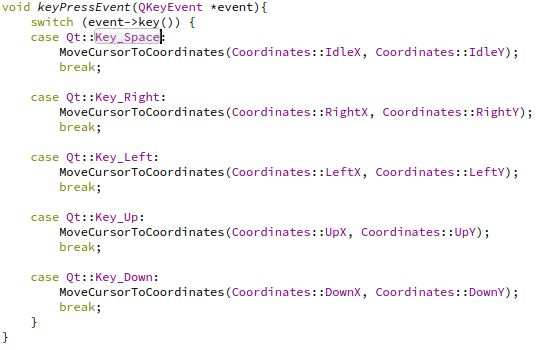
\includegraphics[width = 0.85\textwidth]{keyPressEvent.JPG}
	\caption{MainWindow KeyPressEvent, til test af GUI funktionalitet}
	\label{KeyPressEvents}
\end{figure}

Hvert valgfelts koordinatsæt er aflæst og indsat i et struct i MainWindow, som ses på figur \ref{Coordinates}.

\begin{figure} [H]
	\centering
	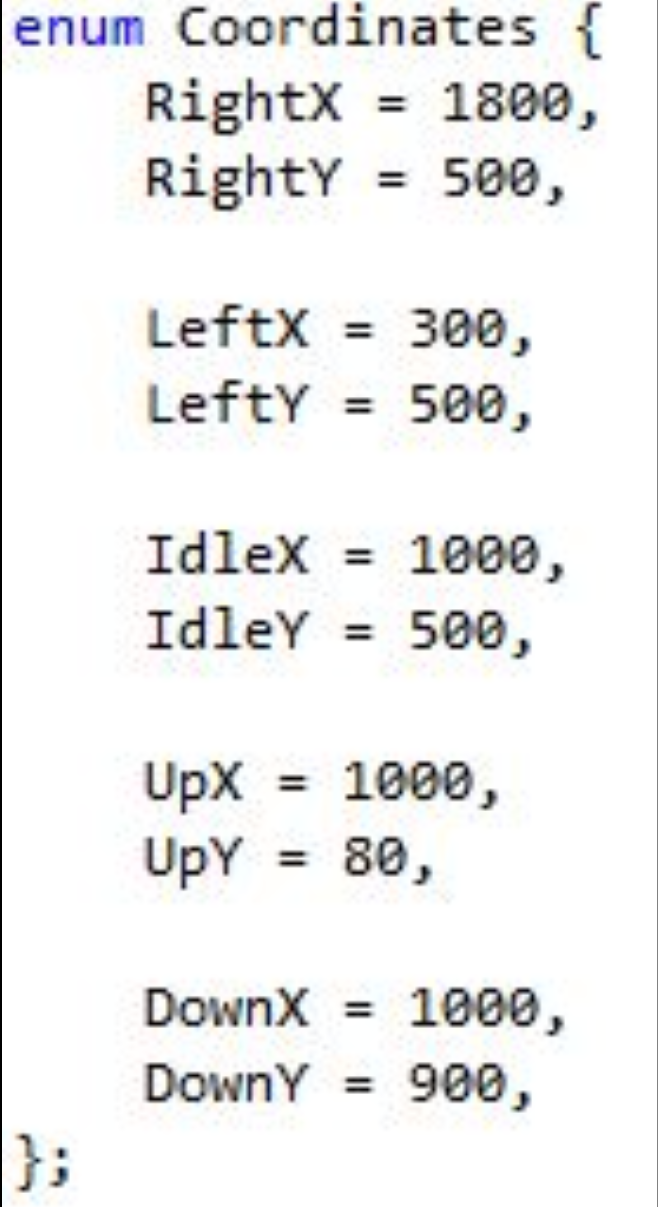
\includegraphics[width = 0.3 \textwidth]{Coordinates.png}
	\caption{Valgfelters koordinatsæt}
	\label{Coordinates}
\end{figure}

I testen ses det, at main modtager en besked om, at det respektive valgfelt er blevet valgt, ud fra input fra piletasterne.